% Introduction

\chapter{Introduction} % Main chapter title

\label{Chapter1} % Change X to a consecutive number; for referencing this chapter elsewhere, use \ref{ChapterX}

%----------------------------------------------------------------------------------------
%	SECTION 1
%----------------------------------------------------------------------------------------

\section{State of VR}

In recent years VR (Virtual Reality) has become widely accessible with the advent of sub-1000\$, enthusiast-grade headsets such as the HTC VIVE and the Occulus Rift, followed by the adoption from a major console platform PlayStation with the PSVR and a slew of low-cost, smartphone-based mobile offerings from startups. On the software front Microsoft is working on Windows Mixed Reality and the two major mobile OSes Android and iOS both have launched developer kits for AR (Augmented Reality) and VR.
\\\\
Whereas in the past there has been a focus on cutting down cost with breakthroughs in hardware, inside-out VR has become an emerging trend this year. This is evident from CES (Consumer Electronics Show) 2017 with many companies showcasing their inside-out VR solutions. The term inside-out refers to how the headset position is tracked. In contrast to outside-in VR which require external sensor arrays for point of reference, inside-out VR only uses on-board sensor without the need of external systems. This is achieved by monocular or binocular visual SLAM (Simultaneous Localization and Mapping) complemented with IMU (Inertial Measurement Unit) sensors. The technology is expected to trickle-down to consumers in few years.

%----------------------------------------------------------------------------------------
%	SECTION 2
%----------------------------------------------------------------------------------------

\section{Gait Analysis}

Gait analysis is a heavily researched topic in many disciplines. From medical sciences including physiology, pathology and gerontology to computer animation and pedestrian tracking, there has been numerous research on this topic. Medical science is where human gait has been extensively studied and where most of the terminology originates from. Research interests range from enhancing the performance of athletes to diseases prediction and rehabilitation. In computer animation gait analysis is used to achieve natural perceived motion in techniques such as motion blending and motion warping which manipulates existing motion capture data to generate motion. Pedestrian tracking requires gait analysis to detect steps and accurately measure stride length.

\newpage
%-----------------------------------
%	SUBSECTION 1
%-----------------------------------
\subsection{Gait Event Detection}
Most commonly recognized gait events are heel-strike, foot-flat, heel-off and toe-off which is well represented in a figure from a book by \cite{Whi06} (Figure \ref{fig:gait_event_whittle}). Heel-strike is when the foot impacts the ground followed by foot-flat when the foot has made full contact with the ground. Subsequent events heel-off and toe-off occurs when the foot is detached from the ground heel to toe.

\begin{figure}[th]
\centering
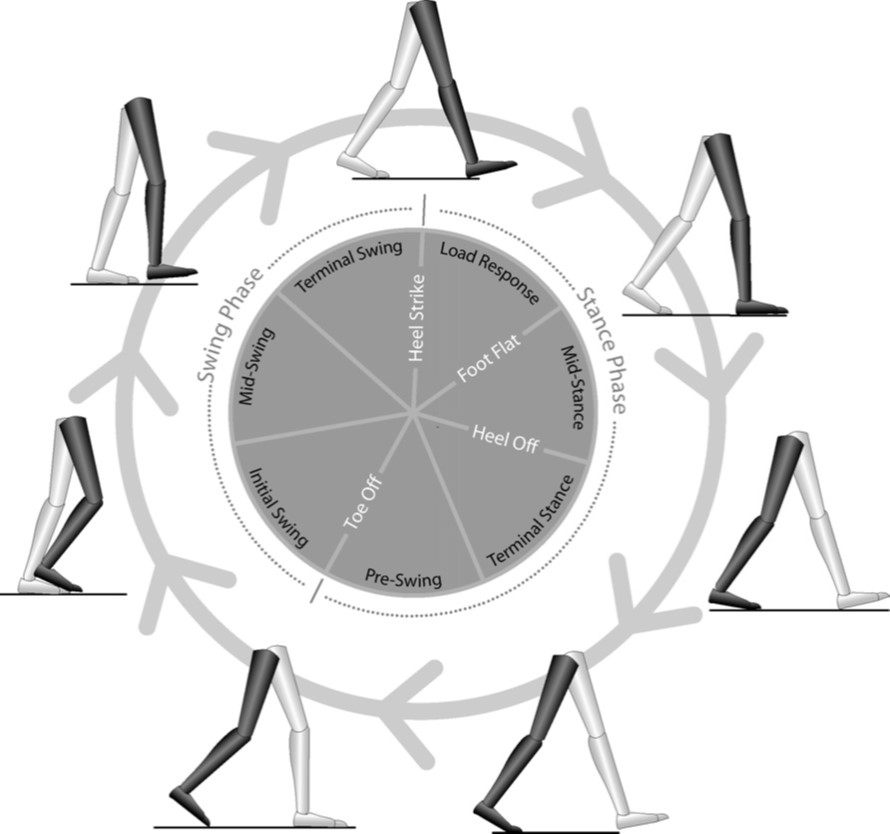
\includegraphics[width=\textwidth,height=\textheight,keepaspectratio]{Figures/gait_event_whittle.jpg}
\decoRule
\caption[Gait event definition]{Gait events as defined in \cite{Whi06}}
\label{fig:gait_event_whittle}
\end{figure}
\noindent
There are various gait event detection methods with different types of sensors and sensor configurations. This is well-documented in a meta-analysis by \cite{Rue10}. In most cases, recent research on gait analysis utilize either force-based sensor, IMU sensor, magnetometer or some combination of aforementioned devices to detect gait events. While it is also possible to obtain gait events from motion capture systems such as the VICON or from depth cameras, these devices are overly sophisticated for the sole purpose of gait event detection.
\\\\
Force-based sensors which measure ground reaction force, range from simple on-off switches to pressure sensitive sensors either in a standalone mat form factor or embedded within the shoe. MEMS (Micro-Electro-Mechanical Systems) IMU sensors and magnetometers are often packaged onto a single board and measure acceleration, angular velocity and magnetic field. Acceleration data is well suited for detecting shocks resulting from contact such as the heel-strike event. For functional analysis angular velocity data is preffered as angular velocity magnitude is invariant to sensor placement, under the reasonable assumption that the sensor is attached to a rigid body (i.e. shoe). Magnetometers can be prone to local magnetic disturbances, especially so in an indoor settings and must be used with caution. Detailed description of gait event detection using IMU sensors is presented by \cite{Jas06}.
\\\\
Different techniques can be deployed to detect gait events from sensor data.  \cite{Rue10} presents a summary of commonly used gait detection methods. With force-based sensors simple thresholding can get the job done. In many cases, functional analysis of either raw sensor data or derived data coupled with FSM (Finite State Machine) can provide reliable gait event detection. With the recent explosion of various learning techniques, data-driven approach  can outperform traditional techniques in some cases.

%-----------------------------------
%	SUBSECTION 2
%-----------------------------------

\subsection{Gait Feature Extraction}
Gait features can be classified into two categories: spatio-temporal and kinematic. The former is represented by a single parameter and the latter is represented by a time series or a waveform. Spatio-temporal features are parameters pertaining to space (spatial) and time (temporal). Spatial parameters include but not limited to step length, stride length, clearances (e.g. MTC, minimum toe clearance), maximum and minimum heights. Temporal parameters include but not limited to cadence, speed and duration between gait events. Kinematic features can be any time series or waveform related to gait that may or may not be represented by wavelets. Kinematic features include but not limited to time series of joint angles, limb angular velocity and limb acceleration.
\\\\
Focusing on IMU-based gait feature extraction techniques, the traditional approach is to obtain gravity-compensated accelerometer data represented in the ground frame with the knowledge of sensor orientation and perform successive integration with constraints provided by gait events to obtain drift-compensated velocity and position \citep{Ram15, Kit16}. Recently there has been data-driven approach to extract gait features directly from IMU sensor data with deep convolutional neural networks \citep{Han17}. If the successive stride vectors can be reliably measured and the initial position is given, PDR (Pedestrian Dead Reckoning) is possible. A detailed overview on this topic is provided by \cite{Woo10}. State of the art PDR algorithm considers heel-strike and toe-off phase and improves upon conventional INS-EKF-ZUPT (Inertial Navigation System - Extended Kalman Filter - Zero Velocity Update) algorithm \citep{Ju16}.
\\\\
For the purpose of this research, spatio-temporal parameters are needed. \cite{Kit16} presents a reliable method to obtain foot trajectory with IMU sensors only. It relies on double integration of the gravity-compensated and orientaion-corrected acceleration with some strong assumptions on the underlying motion to eliminate drift. For gait feature extraction, this research largely adopts the method described in \cite{Kit16}. 

\newpage
%----------------------------------------------------------------------------------------
%	SECTION 3
%----------------------------------------------------------------------------------------

\section{Locomotion Generation in VR}

There are various locomotion generation schemes depending on the input used and the system setup. Inputs include but not limited to gamepad or joystick inputs, headset positional tracking, gesture inputs such as tapping, gaze inputs in stare-to-move and look-down-to-move techniques, WIP (Walking-In-Place) and RDW (Redirected Walking, \cite{Raz01}). A brief taxonomy of techniques is presented by \cite{Nil16} (Figure \ref{fig:taxonomy}).

\begin{figure}[th]
\captionsetup{justification=raggedright,singlelinecheck=false}
\centering
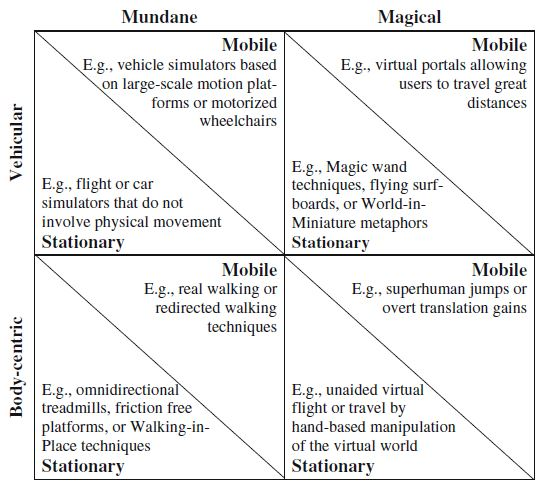
\includegraphics{Figures/taxonomy.jpg}
\decoRule
\caption[Taxonomy of virtual travel techniques]{Taxonomy of virtual travel techniques presented by \cite{Nil16}}
\label{fig:taxonomy}
\end{figure}
\noindent
One of the strong selling points of WIP techniques over headset positional tracking is that the user can navigate infinite virtual space within a limited physical space. Compared with other techniques, WIP techniques provide a interface that is most similar to real walking which is more natural and may alleviate VR sickness. One can argue that RDW which extends the size of the virtual space from a given physical space while retaining the benefits of real walking strikes a nice balance between WIP techniques and headset positional tracking. However, virtual environments have to be designed in such a way that the user following a slightly curved path is convinced to be walking in a straight line without inducing VR sickness. This research seeks to improve upon existing WIP techniques by achieving similar performance with low-cost, inside-out, lightweight IMU-based setup.

\newpage
%-----------------------------------
%	SUBSECTION 1
%-----------------------------------

\subsection{WIP Techniques}
Earlier attempts to synthesize locomotion in VR from WIP motion date back to the 1990s. Surprisingly, earlier attempts include using feed-forward neural networks to determine whether or not the participant is performing WIP motion  \citep{Sla95}. Though the reported accuracy of around 90\% may not be adequate for pratical use. In the last decade there has been resurgence of research on this topic. \cite{Fea08} focused on improving two performance criterion - latency and smoothness (LLCM-WIP, Low-Latency-Continuous-Motion WIP). This was followed by GUD-WIP (Gait-Understanding-Driven WIP) which aimed to generate actual walking-like velocity profile with the knowledge of gait characteristics \citep{Wen10}. \cite{Bru13} improved upon GUD-WIP by using maximum heel height (amplitude) as a metric of locomotion speed and claims less travel time over long distances and improved accuracy in short distances when compared to GUD-WIP (SAS-WIP, Speed-Amplitude-Supported WIP).
\\\\
LLCM-WIP emphasizes low starting/stopping latency and smoothness of the generated locomotion. Heel height signal of left and right foot is conditioned with numerical differentiation, smoothing, DC-bias removal, scaling, etc. which is then summed to be the locomotion speed. Heel height is obtained from magnetic foot trackers. Orientation of the locomotion velocity vector is determined by the chest-orientation tracker. Such implementation, as mentioned by the authors, is prone to magnetic disturbances.
\\\\
Whereas LLCM-WIP relied on signal conditioning of heel height to generate locomotion, GUD-WIP analyzes gait event sequences of walking motion and WIP motion and comes up with a rather sophisticated FSM-based locomotion scheme. The authors claim a smoother, more natural locomotion over LLCM-WIP. However, due to the inherent limitation of state machines, stopping latency is worse than that of LLCM-WIP. GUD-WIP was implemented with optical trackers.
\\\\
SAS-WIP attempts to improve the user experience of the WIP technique by proving the user with more control over locomotion speed which results in reduced user fatigue and better accuracy. Performance is improved (faster long distance travel and more precise short distance travel) over GUD-WIP. SAS-WIP was also implemented with optical trackers.
\\\\
Recently smartphone-based mobile solutions have emerged. Such solutions require minimal hardware and while they may not be as sophisticated as solutions with dedicated hardware, they are more than capable of performing simple functions. \cite{Tre16} synthesizes gaze-directed locomotion when resulting head bobbing motion from WIP triggers an event. Numerous related software packages exist such as the assets found on the Unity Asset Store with varying degrees of success.

\newpage
%----------------------------------------------------------------------------------------
%	SECTION 4
%----------------------------------------------------------------------------------------

\section{Sensor Fusion Orientation Filter}

Orientation can be obtained from multiple sensor data. Accelerometer data provide pitch and roll angles by measuring the direction of gravitational acceleration. Gyroscope data provide orientation relative to initial configuration by integrating angular velocity. Magnetometer data provide a reference direction for yaw angle. Due to sensor characteristics, each has its own strengths and weaknesses. Orientation obtained from accelerometer data is fast and responsive but cannot provide yaw angle and also prone to disturbances such as linear acceleration. Gyroscope data can provide rotations in all directions but is prone to drifting from the integration process. Magnetometer data provide reference heading but more often than not magnetic disturbances, especially in indoor settings, require special consideration.
\\\\
It is common to combine the data from various sensors with sensor fusion algorithms to obtain responsive and robust orientation. IMU-based sensor fusion algorithms require accelerometer and gyroscope data and is used when absolute heading is not required and slight yaw drift is allowed. MARG (Magnetic Angular Rate Gravity) filters incorporate magnetometer data in addition to IMU data to determine the absolute heading but may under-perform compared to IMU filters under high magnetic noise environments. These filters can be implemented with Kalman filters or their variants which is the most widely used approach. Kalman filters require matrix computation which can be computationally expensive. Quaternion-based, gradient descent based orientation filter has been suggested to overcome this computational disadvantage \citep{Mad11}. In this research, Madgwick's algorithm implemented in C was repackaged into C++ class and used to obtain orientation quaternion from IMU sensor data.
